% begin module net-change-physics
\begin{frame}
\begin{itemize}
\item  If an object moves along a straight line with position function $s(t)$, then its velocity is $v(t) = s'(t)$.
\item  In this case, the Net Change Theorem says
\[
\int_{t_1}^{t_2} v(t) \diff t = s(t_2) - s(t_1).
\]
\item<2->  This is the displacement, or net change of position.
\item<3->  If we want to calculate the distance the object travels, we have to consider separately the intervals where $v(t) \geq 0$ (object moves to the right) and $v(t) \leq 0$ (object moves to the left).
\end{itemize}
\vspace{-.5cm}
\begin{columns}
\column{.55\textwidth}
\uncover<4->{%

\psset{xunit=0.8cm, yunit=0.8cm}
\begin{pspicture}(-5, -5)(5,5) 
\psframe*[linecolor=white](-5,-5)(5,5) 
\psaxes[ticks=none, labels=none]{<->}(0,0)(-1.5,-2)(4.7,2.5)\tiny
%Function formula: 4 (x)+1/2 ((x)^{3})-3 ((x)^{2}) 
\pscustom*[linecolor=cyan]{ 
\psplot[linecolor=red, plotpoints=1000]{4}{4.4}{x 2 exp -3 mul x 3 exp 0.5 mul x 4 mul add add } 
\psline(4.4,0)(4,0)
}
%Function formula: 4 (x)+1/2 ((x)^{3})-3 ((x)^{2}) 
\pscustom*[linecolor=orange]{ 
\psplot[linecolor=red, plotpoints=1000]{2}{4}{x 2 exp -3 mul x 3 exp 0.5 mul x 4 mul add add } 
\psline(4,0)(2,0)
}
%Function formula: 4 (x)+1/2 ((x)^{3})-3 ((x)^{2}) 
\pscustom*[linecolor=cyan]{ 
\psplot[linecolor=red, plotpoints=1000]{0.1}{2}{x 2 exp -3 mul x 3 exp 0.5 mul x 4 mul add add }
\psline(2,0)(0.1,0)
}
\psplot[linecolor=red, plotpoints=1000]{0.1}{4.4}{x 2 exp -3 mul x 3 exp 0.5 mul x 4 mul add add }
\psline(0.1, -0.1)(0.1, 0.1)
\psline(4.4, -0.1)(4.4, 0.1)
\rput[t](0.1, -0.15){$t_1$}
\rput[t](4.4, -0.15){$t_2$}
\rput(2, 1){$v(t)$}
\rput (1, 0.5){$A_1$}
\rput (3, -0.5){$A_2$}
\rput[l] (4.2, 0.5){$A_3$}
\end{pspicture} 
%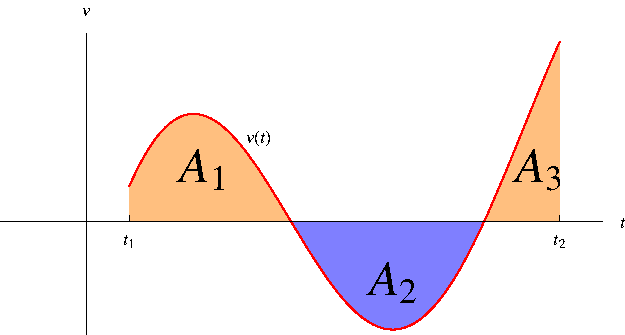
\includegraphics[width=6cm]{integration/pictures/05-04-distance.pdf}
}%
\column{.45\textwidth}
\abovedisplayskip=0pt
\belowdisplayskip=0pt
\abovedisplayshortskip=0pt
\belowdisplayshortskip=0pt
\uncover<4->{%
\begin{align*}
\text{displacement} & =  \int_{t_1}^{t_2} v(t) \diff t\\
& =  A_1 - A_2 + A_3\\
\text{distance} & =  \int_{t_1}^{t_2} |v(t)| \diff t\\
& =  A_1 + A_2 + A_3\\
\end{align*}
}%
\end{columns}
\end{frame}
% end module net-change-physics
